\documentclass[10pt]{article}
\usepackage{multicol}
\usepackage{graphicx}
\usepackage{subcaption}
\usepackage{float}
\usepackage{url}
\usepackage[margin=1.0in]{geometry}
\usepackage[compact]{titlesec}
\titlespacing{\section}{0pt}{5pt}{5pt}
\titlespacing{\subsection}{0pt}{5pt}{5pt}
\titlespacing{\subsubsection}{0pt}{5pt}{5pt}

\titlespacing{\subsubsection}{0pt}{5pt}{5pt}

\title{Node Embeddings for Botnet Detection}
\author{
	Brinton, Joseph\\
	\texttt{jcbrinton@gmail.com}
	\and
	Harker, Christopher\\
	\texttt{chris.harker77@gmail.com}
	\and
	Zhao, Jack\\
	\texttt{u1129777@utah.edu}
}

% Your report must be 3 pages long. You must use a two-column format, 10-point times new roman font, and your lines/paragraphs must be single-spaced. Your report must not include any code. However, you must make your code available on a web page or a repository and provide the pointer to that page in your report.

\begin{document}
\maketitle

\begin{multicols}{2}

% Introduction - Motivate and introduce the problem you are solving. Very briefly summarize your methodology, your experiments, and your important results.
\section{Introduction}

Botnets are a significant source of network attacks, consisting of several compromised computers capable of performing coordinated attacks, including DDoS attacks, click-fraud scams, spamming, and identity theft. A key component in preventing attacks from botnets requires methods to detect them.

Modern botnet detection methods still primarily rely on heuristics built on the manual analysis of traffic patterns, malware code, etc. Machine learning approaches help automate the process, relieving some of the manual labor placed on analysts while showing promise in their ability to detect botnets. However, most machine learning algorithms require inputs defined in the euclidean domain. Therefore, when used on network data, machine learning algorithms fail to take into account crucial relational information between nodes in the network. 

Our project involves studying the node embeddings produced by two of the most commonly used graph embedding algorithms, DeepWalk and Node2Vec. Botnets generally have different structural properties than background networks. For example, centralized botnets have a strong hierarchical structre, while decentralized botnets are designed for efficient diffusion of information. If the botnet has different structural properties than the other nodes in the network, the node embeddings produced by DeepWalk and Node2Vec should be different than nodes elsewhere in the network. 

We trained both DeepWalk \cite{Perozzi} and Node2Vec \cite{Grover} on two scenarios provided as part of the CTU-13 \cite{Garcia} dataset, both of which contain an IRC botnet. The embeddings of nodes in the botnet produced by both algorithms are compared to the embeddings of normal and background nodes by visually inspecting them as well as examining the pointwise euclidean and cosine distances between them. We find that both of these algorithms produce botnet embeddings that are reasonably different from other nodes in the network. 

We also trained DeepWalk on the Aposemat \cite{IoT-23} dataset, which contains three botnets: Mirai, Okiru and Torii. However, DeepWalk failed to produced botnet embeddings that are reasonably different from other nodes in the network.

All of the results presented here as well as additional analysis can be found online at \url{https://github.com/printfer/CS6490_NetworkSecurity_FinalProject}

% Related work - Summarize the existing work related to your problem
\section{Related Work}

Representation Learning was popularized in Natural Language Processing \cite{Camacho},\cite{Madelbaum}. Interestingly, words that are similar to each other have similar embeddings while dissimilar words have dissimilar embeddings. The introduction of the word2vec Skip-gram model \cite{Mikolov} provided more efficient and accurate vector representations.  Researchers have applied these techniques in other networks, especially in biomedical networks \cite{Perkins},\cite{Yue}.

Node embeddings have been used in the context of network security, generally as features in supervised learning problems \cite{Skorniakov}. To the best of our knowledge, however, there is not any research examining the node embeddings themselves. We aim to close this gap, hoping that node embeddings of nodes inside the botnet are similar to each other and dissimilar from nodes elsewhere in the network.

% Methodology
\section{Methodology}

% Adversary model - Describe the adversary you are securing against.
\subsection{Adversarial Model}
In scenarios 10 and 11 in the CTU-13 dataset, it is assumed that the adversary is capable of performing DDoS attacks. Specifically, the adversary uses an IRC protocol and is capable of performing either UDP or ICMP flood attacks \cite{Garcia}. In the IoT-23 dataset, the Mirai botnet has a C2 structure and uses UDP, HTTP, or TCP flooding. Okiru is a Mirai variant and the same model is assumed. The Torii botnet also has a C2 structure but uses telnet flooding attacks.

\subsection{Data}
We utilize two botnet scenarios provided as part of the CTU-13 dataset \cite{Garcia}. This dataset provides large captures of real botnet traffic mixed with normal traffic and background traffic. Each of the thirteen scenarios included in the dataset have different characteristics. We focus on scenario 10 and scenario 11, both of which are IRC botnets performing DDoS attacks. Scenario 10 contains 10 nodes in the botnet, which is performing a UDP DDoS attack, and contains 6 normal nodes. Scenario 11 contains three nodes in the botnet, which is performing a ICMP DDoS attack, and contains six normal nodes. All other IPs in each dataset are background nodes. Using this flow data, we constructed a graph by placing an edge between any two IPs where there was a packet sent between them. 

Another dataset we use is the IoT-23 dataset \cite{IoT-23}. This dataset contains multiple types of malicious IoT network traffic in addition to botnets. As a result of that, the total size of this dataset is huge and it requests a tremendous computing time to process and train. Therefore, we try to reduce the dataset first before train the model. We separate the dataset into small groups and use some basic statistic techniques to count which part has the densest botnet and use that part for our final training. Finally, we use scenarios pertaining to the Mirai, Okiru, and Torii botnets. 

\subsection{Algorithms}
 \subsubsection{DeepWalk}
DeepWalk \cite{Perozzi} was inspired by methods used in natural language modeling in which vector representations of words are produced by estimating the likelihood that a sequence of context words appear given a root word. In DeepWalk, ``sentences" of nodes are generated by generating random walks on a graph and then maximizing the probability that the nodes appear given the source node. However, the probabilities are never used. Rather, a mapping function that maps a node to its latent representation and is learning during training is used as the embeddings. Specifically, the embeddings are generated by training a Skip-gram model \cite{Mikolov}, \cite{Perozzi}.

\subsubsection{Node2Vec}
Node2Vec \cite{Grover} is similar to DeepWalk in the sense that it trains a Skip-gram model by using random walks on the graph. It differs from DeepWalk, however, in how the random walks are generated. Instead of selecting any of its neighbors uniformly at random as the next node in the walk, Node2Vec uses two hyperparameters to weight the edges, making some nodes more likely to be selected than others. Depending on the values of these two hyperparameters, the random walks emphasize the local structure around a node or a more global structure. 

% Implementation/Experimentation - Describe your experiments and your results. Discuss your results.
\section{Experiments and Discussion}
\subsection{CTU-13 Dataset}

Both DeepWalk and Node2Vec were trained on scenario 10 and scenario 11 from the CTU-13 dataset. DeepWalk was run using several different combinations of hyperparameters then the embeddings were inspected visually. Node2Vec, however, was only run on one set of hyperparameters due to the algorithm being computationally expensive. Similarly, Node2Vec was only run on scenario 11 because of memory limitations  that arise when run on scenario 10.

We analyzed the similarity between botnet nodes and normal/background nodes by calculating the pairwise euclidean and cosine distances between them. The pairwise euclidean distance between embeddings produced by DeepWalk on scenario 10  are shown below in Figure 1. As we can see, the nodes inside the botnet are very similar to each other while being visibly different from the normal nodes. The distance between botnet nodes and background nodes are even more pronounced and the results can be found online.


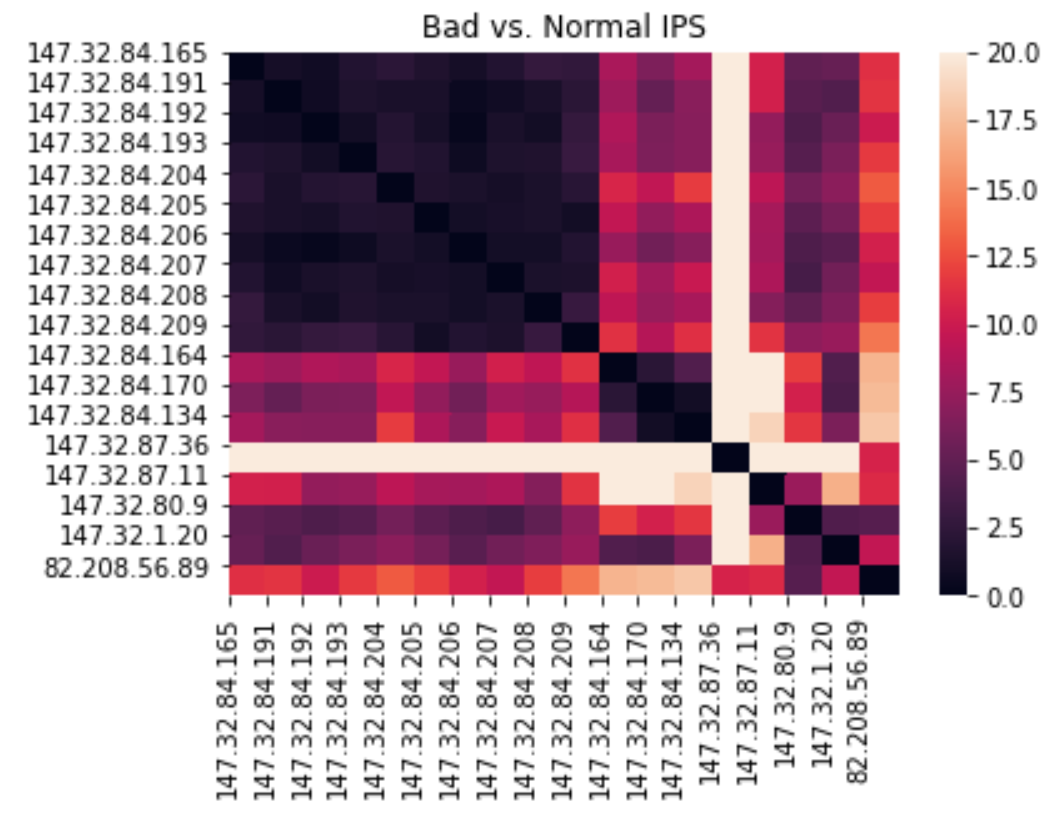
\includegraphics[scale=0.7]{1a.png}
\captionof{figure}{Pairwise euclidean distance of DeepWalk embeddings of scenario 10.\newline}

We performed a similar analysis on scenario 11 using both DeepWalk and Node2Vec. DeepWalk produces results similar to those of scenario 10, where there is a visible difference between the bad nodes from the normal nodes. The embeddings produced by Node2Vec might capture the structural differences even better than DeepWalk does. We were only able to try one set of hyperparameters for Node2Vec so even better embeddings might be produced if we had more time to try more combinations of hyperparameters. \newline

%\begin{figure}[H]
%\centering
%\begin{subfigure}[b]{0.55\textwidth}
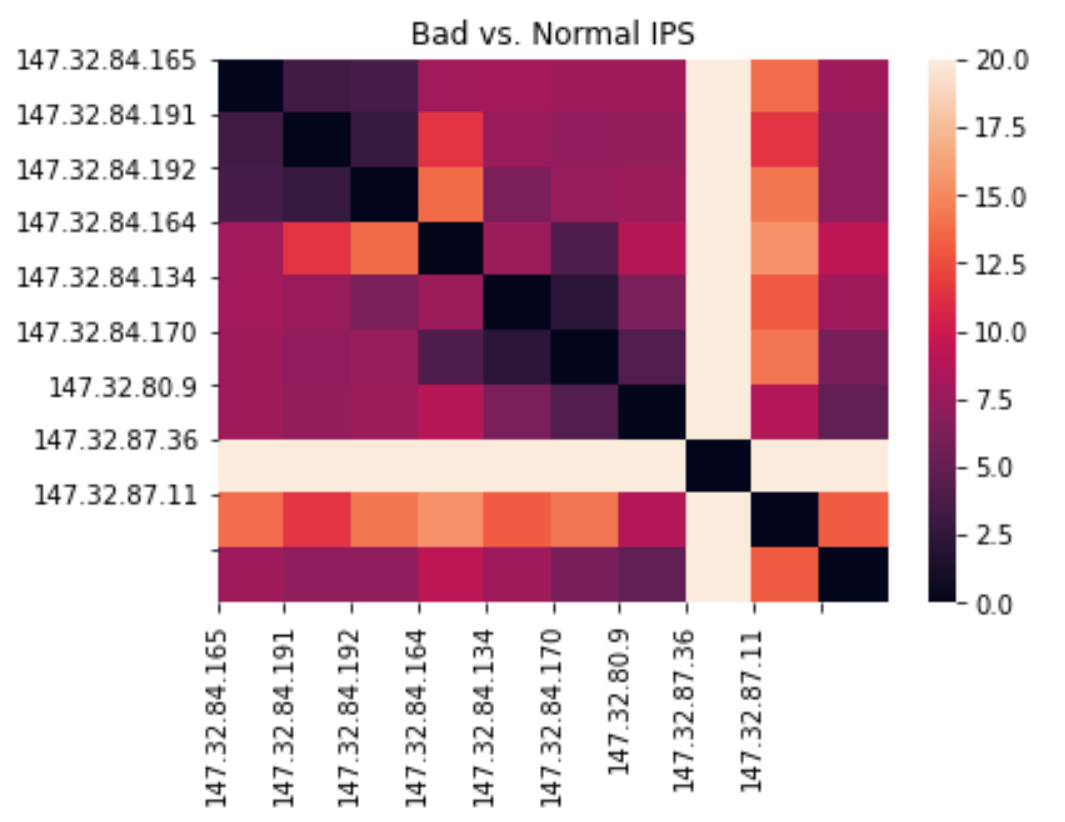
\includegraphics[scale=.7]{2a}
\captionof{figure}{Pairwise euclidean distance of DeepWalk Embeddings of scenario 11.\newline}

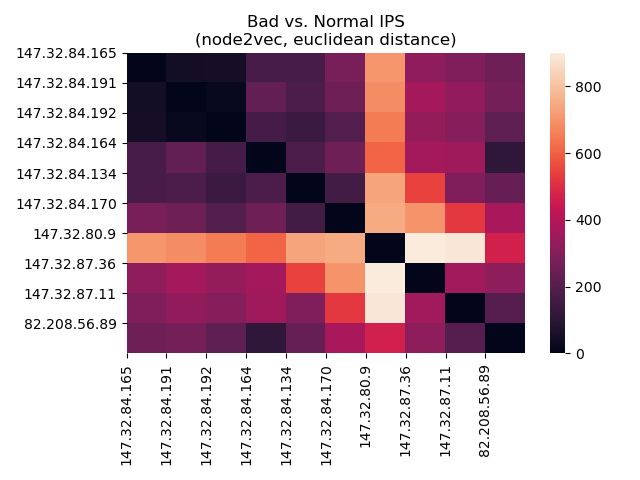
\includegraphics[scale=.5]{2b}
\captionof{figure}{Pairwise euclidean distance of Node2Vec Embeddings of scenario 11.\newline}

%\end{figure}

\subsection{IoT-23 Dataset}

We performed a similar analysis of Deepwalk embeddings on the IoT-23 Dataset. However, the embeddings do not give as clear of a result as the CTU-13 embeddings. We use the similar techniques as before and analyzed the similarity between botnet nodes and normal/background nodes by calculating the pairwise euclidean and cosine distances between them. However, the nodes in the botnet do not appear to be any more similar to each other compared to nodes elsewhere in the network. This could be due to the Mirai botnet having a structure that is more difficult to capture, the fact that the Mirai botnet is more sophisticated and its traffic appears more like normal traffic better than botnets in CTU-13. We were also only able to try one set of hyperparameters due to computational limitations. Other combinations of parameters may produce better results. 

% Conclusion - Summarize your work and your results. Indicate any future directions.
\section{Conclusion}

Using two scenarios from the CTU-13 dataset, we trained DeepWalk and Node2Vec embeddings. We compared the embeddings of nodes in the botnet against other nodes in the network. This was done by calculating the pairwise euclidean distance between them. The DeepWalk embeddings of botnet nodes differ from other nodes significantly enough that the differences can be seen visually, suggesting that DeepWalk embeddings adequately captures the structural differences and similarities between nodes and can possibly be used to identify botnets within networks. However, for more sophisticated IoT botnets such as Mirai the results are not as clear. \newline

Future work might include searching over a wider space of hyperparameters in order to examine if there exists a combination that produces better embeddings, especially for the more computationally expensive Node2Vec. Also, we might explore the embeddings of botnets that have different structures, such as P2P botnets and other IoT botnets. 

\begin{thebibliography}{5}

\bibitem{Camacho}
Camacho-Collados, Jose and Pilehvar, Mohammad Taher.
\textit{From Word to Sense Embeddings: A Survey on Vector Representations.}
arXiv. 2018.
\texttt{https://arxiv.org/abs/1805.04032}

\bibitem{Garcia}
Garcia, Sebastian and Grill, Martin and Stiborek, Jan and Zunino, Alejandro.
\textit{An empirical comparison of botnet detection methods.}
Computers and Security Journal, Elsevier. 2014. Vol 45, pp 100-123.
\texttt{http://dx.doi.org/10.1016/j.cose.2014.05.011}

\bibitem{Grover}
Grover, Aditya and Leskovec, Jure.
\textit{node2vec: Scalable Feature Learning for Networks}
ACM SIGKDD International Conference on Knowledge Discovery and Data Mining, ACM Press. 2016.
\texttt{https://arxiv.org/abs/1607.00653}

\bibitem{Madelbaum}
Madelbaum, Amit and Shalev, Adi.
\textit{Word Embeddings and Their Use in Sentence Classification Tasks.}
arXiv. 2016. 
\texttt{https://arxiv.org/abs/1610.08229}

\bibitem{Mikolov}
Mikolov, Tomas and Sutskever, Ilya and Chen, Kai and Corrado, Greg and Dean, Jeffrey.
\textit{Distributed Representations of Words and Phrases and Their Compositionality.}
Proceedings of the 26th International Conference on Neural Information Processing Systems, Curran Associates Inc. 2013. Vol 2, pp 3111-3119.
\texttt{https://dl.acm.org/doi/10.5555/2999792.2999959}

\bibitem{Perkins}
Perkins, James and Diboun, Ilhem and Dessailly, Benoit and Lees, Jon and Orengo, Christine.
\textit{Transient Protein-Protein INteractions: Structural, Functional, and Network Properties.}
Structure. 2010. Vol. 18, Iss. 10, pp 1233-1243.
\texttt{https://doi.org/10.1016/j.str.2010.08.007}

\bibitem{Perozzi}
Perozzi, Bryan and Al-Rfou, Rami and Skiena, Steven.
\textit{DeepWalk: Online Learning of Social Representations.}
Proceedings of the 20th ACM SIGKDD International Conference on Knowledge Discovery and Data Mining, ACM Press. 2014.
\texttt{http://dx.doi.org/10.1145/2623330.2623732}

\bibitem{Skorniakov}
Skorniakov, Kirill and Turdakov, Denis and Zhabot, Andrey.
\textit{Make Social Networks Clean Again: Graph Embedding and Stacking Classifiers for Bot Detection.}
CIKM Workshops. 2018.
\texttt{http://ceur-ws.org/Vol-2482/paper39.pdf}

\bibitem{Yue}
Yue, Xiang and Wang, Zhen and Huang, Jingong and Parthasarathy, Srinivasan and Moosavinasab, Soheil and Huang, Yungui and Lin, Simon and Zhang, Wen and Zhang, Ping and Sun, Huan.
\textit{Graph Embedding on Biomedical Networks: Methods, Applications and Evaluations.}
Bioinformations. 2020. Vol. 36, Iss. 4, pp 1241-1251.
\texttt{https://doi.org/10.1093/bioinformatics/btz718}

\bibitem{IoT-23}
Stratosphere Laboratory.
\textit{A labeled dataset with malicious and benign IoT network traffic.}
January 22th. Agustin Parmisano, Sebastian Garcia, Maria Jose Erquiaga.
\texttt{https://www.stratosphereips.org/datasets-iot23}

\end{thebibliography}

\end{multicols}
\end{document}
